\documentclass{beamer}
\usepackage{amsmath, amssymb}
\usepackage{graphicx}
\usepackage{listings}
\usepackage{color}
\usepackage{tcolorbox,fancyvrb,xcolor,tikz}
\tcbuselibrary{skins,breakable}

\newenvironment{VerbatimIN}
 {\VerbatimEnvironment
  \begin{tcolorbox}[
    breakable,
    colback=lightgray,
    spartan
  ]%
  \begin{Verbatim}}
 {\end{Verbatim}\end{tcolorbox}}

 \newenvironment{VerbatimOUT}
 {\VerbatimEnvironment
  \begin{tcolorbox}[
    breakable,
    spartan
  ]%
  \begin{Verbatim}}
 {\end{Verbatim}\end{tcolorbox}}

\definecolor{darkred}{rgb}{0.75, 0, 0}
\definecolor{orange}{rgb}{1, 0.65, 0}
\definecolor{violet}{rgb}{0.58, 0, 0.83}
\definecolor{darkgray}{rgb}{0.33, 0.33, 0.33}
\definecolor{darkgreen}{rgb}{0.0, 0.5, 0.0}

\title{Mixed Effects Models - Day 5}
\subtitle{Theory of Mixed Effect Models}
\author{Marieke Wesselkamp \\ Department of Biometry and Environmental Systems Analysis \\
Albert-Ludwigs-University of Freiburg (Germany)}
\date{February 2023}

\begin{document}

\frame{\titlepage}


% Slide 2: Linear Effects Model
\begin{frame}{Linear Effects Model in general matrix notation}
\[
\mathbf{y} = \mathbf{X} \cdot \mathbf{b} + \mathbf{e}
\]
\[
\mathbf{e} \sim \mathcal{N}(0, \sigma^2_{\epsilon} \cdot \mathbf{I})
\]
where:
\begin{itemize}
  \item $\mathbf{y}$: measured response values
  \item $\mathbf{X}$: design matrix
  \item $\mathbf{b}$: parameter vector of the design matrix
  \item $\mathbf{e}$: error vector with $mean = 0$, $variance = \sigma^2_{\epsilon} \cdot \mathbf{I}$
  \item $\mathbf{\sigma^2_{\epsilon} \cdot \mathbf{I}}$: error or residual variance-covariance matrix
\end{itemize}
\vspace{0.5cm}

From now on: $\sigma^2_{\epsilon} \cdot \mathbf{I} = \mathbf{R}$ (Residual = R-side).
\end{frame}

% Slide 3: Linear Mixed Effects Model
\begin{frame}{Linear Mixed Effects Model in general matrix notation}
\[
\mathbf{y} = \mathbf{X} \cdot \mathbf{b} + \mathbf{Z} \cdot \mathbf{u} + \mathbf{e}
\]
\[
\mathbf{e} \sim \mathcal{N}(0, \mathbf{R}), \quad \mathbf{u} \sim \mathcal{N}(0, \mathbf{G}), \quad \mathbf{u} \bot \mathbf{e}
\]
where:
\begin{itemize}
  \item $\mathbf{X}$: Fixed Effects design matrix
  \item $\mathbf{b}$: Fixed Effects parameter vector
  \item $\mathbf{Z}$: Random Effects design matrix
  \item $\mathbf{u}$: Random Effects parameter vector
\end{itemize}
\end{frame}

% Slide 5: Matrix Representation of Response
\begin{frame}[fragile]
\frametitle{Let's break it down}
    \large The response vector \textbf{y}
    \begin{columns}
        \begin{column}{0.5\textwidth}        
        \normalsize
            \[
            \mathbf{y} = \left( 
            \begin{array}{c} 
            \color{darkred}{y_1} \\ 
            \color{darkred}{y_2} \\ 
            \color{orange}{y_3} \\ 
            \color{orange}{y_4} \\ 
            \color{violet}{y_5} \\ 
            \color{violet}{y_6} \\ 
            \color{darkgray}{y_7} \\ 
            \color{darkgray}{y_8} 
            \end{array}\right) = \left( 
            \begin{array}{c} 
            \color{darkred}{1.63} \\ 
            \color{darkred}{8.03} \\ 
            \color{orange}{2.68} \\ 
            \color{orange}{0.47} \\ 
            \color{violet}{3.77} \\ 
            \color{violet}{3.76} \\ 
            \color{darkgray}{2.15} \\ 
            \color{darkgray}{5.61} 
            \end{array}\right)
            \]
        \end{column}
        \begin{column}{0.5\textwidth}
            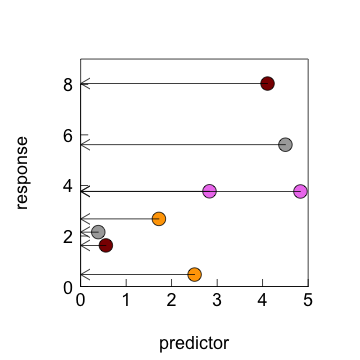
\includegraphics[width=\textwidth]{lectures/day_5_theory_of_mems/figures/unnamed-chunk-3-1.png}
        \end{column}
    \end{columns}
    \vspace{0.3cm}
    
    \large\textbf{4} groups are measured \textbf{2} times each...
\end{frame}

% Slide 6: Fixed Effects Design Matrix
\begin{frame}
\frametitle{Fixed Effects Design Matrix X}
\large ...at two different values of a continous predictor
\begin{columns}
        \begin{column}{0.5\textwidth}
            \[
\mathbf{X} = \left( 
\begin{array}{cc} 
\color{darkred}{1} & \color{darkred}{0.56} \\ 
\color{darkred}{1} & \color{darkred}{4.11} \\ 
\color{orange}{1} & \color{orange}{1.72} \\ 
\color{orange}{1} & \color{orange}{2.51} \\ 
\color{violet}{1} & \color{violet}{2.83} \\ 
\color{violet}{1} & \color{violet}{4.83} \\ 
\color{darkgray}{1} & \color{darkgray}{0.39} \\ 
\color{darkgray}{1} & \color{darkgray}{4.5} 
\end{array}\right)
\]
        \end{column}
        \begin{column}{0.5\textwidth}
            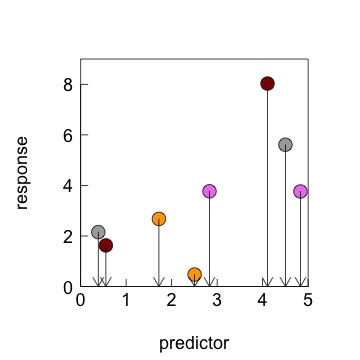
\includegraphics[width=\textwidth]{lectures/day_5_theory_of_mems/figures/unnamed-chunk-4-1.png}
        \end{column}
    \end{columns}

\end{frame}

\begin{frame}
\frametitle{The Parameter Vector b}
    \begin{columns}
        \begin{column}{0.5\textwidth}
\[
\boldsymbol{b} = 
\begin{pmatrix}
\beta_0 \\
\beta_1
\end{pmatrix} =
\begin{pmatrix}
intercept \\
slope
\end{pmatrix}
\]
\[
=
\begin{pmatrix}
0.98 \\
0.48
\end{pmatrix}
\]
        \end{column}
        \begin{column}{0.5\textwidth}
            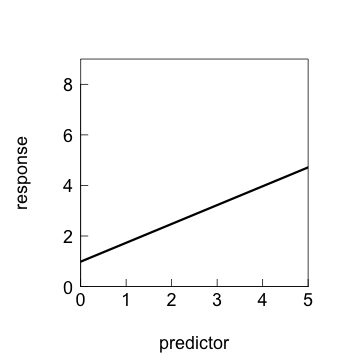
\includegraphics[width=\textwidth]{lectures/day_5_theory_of_mems/figures/unnamed-chunk-5-1.png}
        \end{column}
    \end{columns}
    \vspace{0.3cm}
    
    \large \textit{The parameter vector b describes the average deterministic part of the model}
\end{frame}

% Slide 7: Random Effects Design Matrix
\begin{frame}{Random Effects Design Matrix Z}
\begin{columns}
        \begin{column}{0.5\textwidth}
\[
\mathbf{Z} = \left( 
\begin{array}{cccc} 
\color{darkred}{1} & 0 & 0 & 0 \\ 
\color{darkred}{1} & 0 & 0 & 0 \\ 
0 & \color{orange}{1} & 0 & 0 \\ 
0 & \color{orange}{1} & 0 & 0 \\ 
0 & 0 & \color{violet}{1} & 0 \\ 
0 & 0 & \color{violet}{1} & 0 \\ 
0 & 0 & 0 & \color{darkgray}{1} \\ 
0 & 0 & 0 & \color{darkgray}{1} 
\end{array}\right)
\]
        \end{column}
        \begin{column}{0.5\textwidth}
        \large
            1) There are only 1s because it is a \textbf{Random Intercept} model \\
            \vspace{0.3cm}
            
            2) It is \textbf{sparse} = complete empty elements because of the grouping
        \end{column}
    \end{columns}

\end{frame}

% Slide 8: Random Effects Parameter Vector
\begin{frame}{Random Effects Parameter Vector u}
\large u values as group-specific \textbf{deviations} from the population average intecept $\beta_0$
\begin{columns}
        \begin{column}{0.5\textwidth}
\[
\mathbf{u} = \left( 
\begin{array}{c} 
\color{darkred}{u_1} \\ 
\color{orange}{u_2} \\ 
\color{violet}{u_3} \\ 
\color{darkgray}{u_4} 
\end{array}\right) = \left( 
\begin{array}{c} 
\color{darkred}{0.24} \\ 
\color{orange}{-0.20} \\ 
\color{violet}{-0.12} \\ 
\color{darkgray}{0.09} 
\end{array}\right)
\]
        \end{column}
        \begin{column}{0.5\textwidth}
            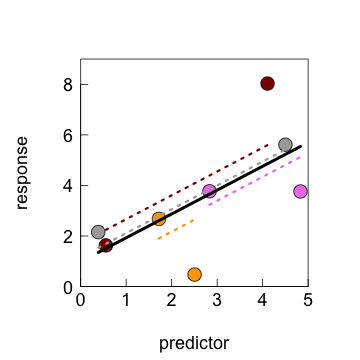
\includegraphics[width=\textwidth]{lectures/day_5_theory_of_mems/figures/unnamed-chunk-6-1.png}
        \end{column}
    \end{columns}
    \vspace{0.2cm}
\large\textit{The random intercepts shift the group-specific lines up or down}
\end{frame}

% Slide 10: Error Vector
\begin{frame}{Error Vector $\epsilon$}
    \begin{columns}
        \begin{column}{0.5\textwidth}
\[
\mathbf{e} = \left( 
\begin{array}{c} 
\color{darkred}{\epsilon_1} \\ 
\color{darkred}{\epsilon_2} \\ 
\color{orange}{\epsilon_3} \\ 
\color{orange}{\epsilon_4} \\ 
\color{violet}{\epsilon_5} \\ 
\color{violet}{\epsilon_6} \\ 
\color{darkgray}{\epsilon_7} \\ 
\color{darkgray}{\epsilon_8} 
\end{array}\right) = \left( 
\begin{array}{c} 
\color{darkred}{-0.12} \\ 
\color{darkred}{2.93} \\ 
\color{orange}{0.27} \\ 
\color{orange}{-2.67} \\ 
\color{violet}{0.23} \\ 
\color{violet}{-1.67} \\ 
\color{darkgray}{0.72} \\ 
\color{darkgray}{0.30} 
\end{array}\right)
\]
        \end{column}
        \begin{column}{0.5\textwidth}
            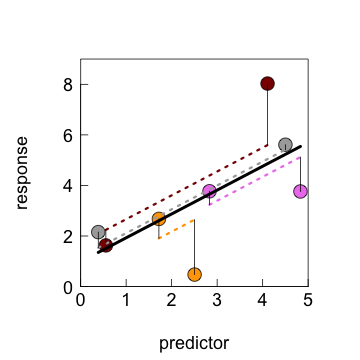
\includegraphics[width=\textwidth]{lectures/day_5_theory_of_mems/figures/unnamed-chunk-7-1.png}
        \end{column}
    \end{columns}
    \vspace{0.3cm}
    
\large \textit{Deviations of the measurements from the random effects values u = the deviations from the deviations}
\end{frame}

% Slide 11: Two Stochastic Parts
\begin{frame}{Two Stochastic Parts in Mixed Models}
\Large
A Mixed Effects Model has two stochastic parts:
\vspace{0.2cm}

\begin{enumerate}
  \item $\mathbf{u} \sim \mathcal{N}(0, \mathbf{G})$ describing how the random effects $\mathbf{u}$ vary around $0$ and is given by the random effects variance-covariance matrix $\mathbf{G}$.
  \item $\mathbf{e} \sim \mathcal{N}(0, \mathbf{R})$ describes how the residuals vary after accounting for fixed and random effects.
\end{enumerate}
\end{frame}

% Slide 12: Random Intercept Model Variance
\begin{frame}{Random Intercept Model Variance}
In the simplest case of a Random Intercept Model, $\mathbf{G}$ has only one value for the variance of random intercepts among groups:
\[
\mathbf{G} = \left( d^2 \right) = 0.29
\]
\end{frame}

% Slide 13: Combined Variance-Covariance Matrix $\mathbf{V}$
\begin{frame}{Combined Variance-Covariance Matrix $\mathbf{V}$}
The combined variance-covariance matrix $\mathbf{V}$ is:
\[
\mathbf{V} = \mathbf{Z} \cdot \mathbf{G} \cdot \mathbf{Z}^T + \mathbf{R}
\]
If $\mathbf{G} = 0$, we are back to the Linear Model.
\end{frame}

% Slide 14: Example of $\mathbf{V}$ Matrix
\begin{frame}{Example of $\mathbf{V}$ Matrix}
For two groups, the $\mathbf{V}$ matrix is:
\[
\mathbf{V} = \left( 
\begin{array}{cc} 
\sigma^2 + d^2 & d^2 \\ 
d^2 & \sigma^2 + d^2 
\end{array} \right)
\]
$d^2$ represents the covariance of two values in the same group.
\end{frame}

% Slide 15: Summary of Assumptions of LMM
\begin{frame}{Assumptions of Linear Mixed Models}
\[
\mathbf{y} = \mathbf{X} \cdot \mathbf{b} + \mathbf{Z} \cdot \mathbf{u} + \mathbf{e}
\]
\[
\mathbf{e} \sim \mathcal{N}(0, \mathbf{R}), \quad \mathbf{u} \sim \mathcal{N}(0, \mathbf{G}), \quad \mathbf{u} \bot \mathbf{e}
\]
Key assumptions:
\begin{itemize}
  \item $\mathbf{b}$ describes the deterministic trend.
  \item $\mathbf{u}$ are normally distributed with mean 0, variance $\mathbf{G}$.
  \item Residual errors $\mathbf{e}$ are independent within a group with variance $\mathbf{R}$.
\end{itemize}
\end{frame}

% Slide 16: Nested vs Crossed Random Effects
\begin{frame}{Nested vs Crossed Random Effects}
When you have two or more random effects in a dataset:
\begin{itemize}
  \item **Nested Random Effects**: Each level of a lower grouping factor is nested within a level of a higher grouping factor.
  \item **Crossed Random Effects**: Random effects are not nested, each level of a grouping factor appears across levels of another factor.
\end{itemize}
\end{frame}

% Slide 17: REML Estimation
\begin{frame}{REML Estimation}
Restricted Maximum Likelihood (REML) is used in Mixed Models to estimate variance components in an unbiased way. REML is preferred when:
\begin{itemize}
  \item Comparing models that differ in their random effects structure.
  \item It adjusts for the fixed effects and focuses on variance components.
\end{itemize}
\end{frame}

% Slide 18: Best Linear Unbiased Predictors (BLUPs)
\begin{frame}{Best Linear Unbiased Predictors (BLUPs)}
Random effects $\mathbf{u}$ are calculated as:
\[
\mathbf{u} = \mathbf{G} \cdot \mathbf{Z}^T \mathbf{V}^{-1} (\mathbf{y} - \mathbf{X} \cdot \mathbf{b})
\]
BLUPs are:
\begin{itemize}
  \item Linear combinations of fixed and random effects.
  \item Unbiased estimates of group-specific trends.
\end{itemize}
\end{frame}

% Slide 19: Shrinkage in Partial Pooling
\begin{frame}{Shrinkage in Partial Pooling}
Mixed effects models use partial pooling to shrink parameter estimates towards the population average. This reduces variance and improves generalization.
\end{frame}

% Slide 20: Recapitulation of Day 5
\begin{frame}{Recapitulation - Day 5}
By the end of today, you should understand:
\begin{itemize}
  \item How a Mixed Effects Model is expressed in matrix notation.
  \item The stochastic part matrices in Linear Mixed Models.
  \item The difference between Random Intercept and Random Slope models.
\end{itemize}
\end{frame}

% Slide 21: Recapitulation of Day 6
\begin{frame}{Recapitulation - Day 6}
After the next session, you will understand:
\begin{itemize}
  \item Nested and Crossed Random Effects.
  \item How to obtain unbiased REML estimates.
  \item The concepts of shrinkage and BLUPs.
\end{itemize}
Have a nice weekend!
\end{frame}

\end{document}